\documentclass{article}
\usepackage{graphicx} % Required for inserting images
\usepackage[parfill]{parskip}
\usepackage{braket}
\usepackage{hyperref}
\usepackage{float}
\usepackage{listings}
\usepackage{xcolor}
\usepackage{multicol}
\usepackage{lipsum}
\usepackage{mwe}

\definecolor{codegreen}{rgb}{0,0.6,0}
\definecolor{codegray}{rgb}{0.5,0.5,0.5}
\definecolor{codepurple}{rgb}{0.58,0,0.82}
\definecolor{backcolour}{rgb}{0.95,0.95,0.92}

\lstdefinestyle{mystyle}{
    backgroundcolor=\color{backcolour},   
    commentstyle=\color{codegreen},
    keywordstyle=\color{magenta},
    numberstyle=\tiny\color{codegray},
    stringstyle=\color{codepurple},
    basicstyle=\ttfamily\footnotesize,
    breakatwhitespace=false,         
    breaklines=true,                 
    captionpos=b,                    
    keepspaces=true,                 
    numbers=left,                    
    numbersep=5pt,                  
    showspaces=false,                
    showstringspaces=false,
    showtabs=false,                  
    tabsize=2
}

\lstset{style=mystyle}

\title{
PYL749 - Quantum Information \& Computing \\ 
Colouring graphs with Quantum Computing
}
\author{Yash Solanki, 2021PH10813}
\date{November 2023}

\begin{document}

\maketitle

\section{Introduction: K-Colourable graphs}

\subsection{Graphs:}

A graph is an ordered pair G = (V, E) such that: 
\begin{itemize}
    \item V is a set of vertices(called Nodes), and 
    \item E $\subseteq$ \{\{x, y\}, x $\in$ V and y $\in$ V\ and x $\neq$ y\}, is the set of edges, an unordered pair \{x, y\}
\end{itemize}
The set E shows the 
association between the vertex pair \{x, y\}. 
\begin{figure}[h]
  \centering
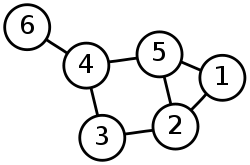
\includegraphics[width=0.5\textwidth]{graph1.png}
  \caption{A graph}
  \label{fig:A graph}
\end{figure}

\subsection{Colouring a graph:}

In graph theory, colouring a graph assigns labels $\forall$ v $\epsilon$ V, such that none of its neighbours has the same label(read: colour). Colouring, as a computational problem, has a large number of practical applications, such as studying networks in electrical engineering, matching in computer science, exam scheduling for institutions and solving Sudoku puzzles for the early birds. K-colouring and bipartite matching are some of the essential concepts used for these applications. 

K-colouring is a colouring of graph G such that different labels/colours are used at exactly' K'. The chromatic number $\chi$(G) denotes the minimum number of colours required to colour a graph. For our application, we will consider the case of K $\geq$ $\chi$(G) or report that it doesn’t exist.

\begin{figure}[h]
  \centering
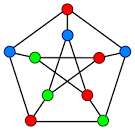
\includegraphics[width=0.5\textwidth]{graph2.png}
  \caption{A 4-coloured graph}
  \label{fig:Coloured graph}
\end{figure}

The above graph is 4-coloured. Interestingly,  any planar graph can be 4-coloured(which is really cool)! In general, K-colouring is an NP-complete problem. Hence, we have to ‘search’ through all the possible solutions to check where a graph is K-colourable and find one such colouring.

\section{Grover’s Algorithm- The Quantum search algorithm:
}

\subsection{Grover's algorithm for one solution:}

Grover’s algorithm is a quantum search algorithm on unstructured(without any known order of constraint) that finds the output with a high probability that a boolean function is satisfied. The time complexity of Grover’s algorithm is $O(N^{1/2})$, where N is the number of elements present in the domain of possible solutions. Since NP-complete problems require an exhaustive search subroutine, we can often speed up the search with Grover’s algorithm.

We have a boolean f: \{0, 1, 2 … N - 1\} $\mapsto$ \{0, 1\} such that f is true for only one value of x in the domain. We then have a subroutine/oracle $U_\omega$ such that:

\begin{itemize}
    \item if f(x) = 1, then $U_\omega$$\ket{x}$ = -$\ket{x}$
    \item if f(x) = 0, then $U_\omega$$\ket{x}$ = $\ket{x}$
\end{itemize}

The algorithm gives x such that f(x) = 1 with a probability of $\geq$ 1/2 for each iteration. We can get arbitrarily large accuracy by running the routine several times. We then invert the amplitudes about the mean frequency, increasing the required x's amplitude and suppressing other values. Measuring the amplitude of states then gives us the required answer.($\pi N ^ {1/2}$)/4 is the approximate number of steps which give us the exact result

More formally, the algorithm follows the following steps:

\begin{itemize}
    \item Initialize the system to the uniform superposition over all states
    \item Perform the subroutine r(N) times. First apply $U_\omega$ followed by $U_s$ = 2 $\ket{s}\bra{s} - I$, called Grover's diffusion operator
    \item Measure the resulting quantum state in the computational basis.
\end{itemize}

The circuit for this algorithm is as follows:

\begin{figure}[h]
  \centering
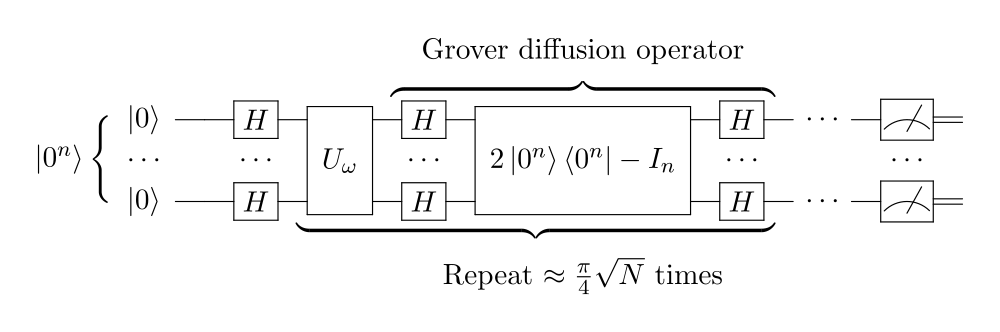
\includegraphics[width=1\textwidth]{grover.png}
  \caption{Quantum Circuit for Grover's algorithm, adapted from [4]}
  \label{Quantum Circuit for Grover's algorithm}
\end{figure}

The main idea behind Grover's algorithm is amplitude amplification of the state for which we are searching. We start with an initial state that is superposition of the domain in which we have to find the solution. This if followed by inverting the amplitude of state which satisfies our constraints. 

These steps are followed by Grover's diffusion, which is equivalent inverting the values about the mean. Since, only the value for which f(x) = 1, the state has a negative phase whereas all other states have a positive phase, inverting about the mean amplifies the negative phase state. Finally, on measuring the state in computational basis, the basis vector with f(x) has the highest probability of being measured.

To make sure that we get the right state upon measurement, we repeat the above subroutine/oracle r(N) times so that the probability of measuring the right state tends to 1.

\begin{figure}[H]
  \centering
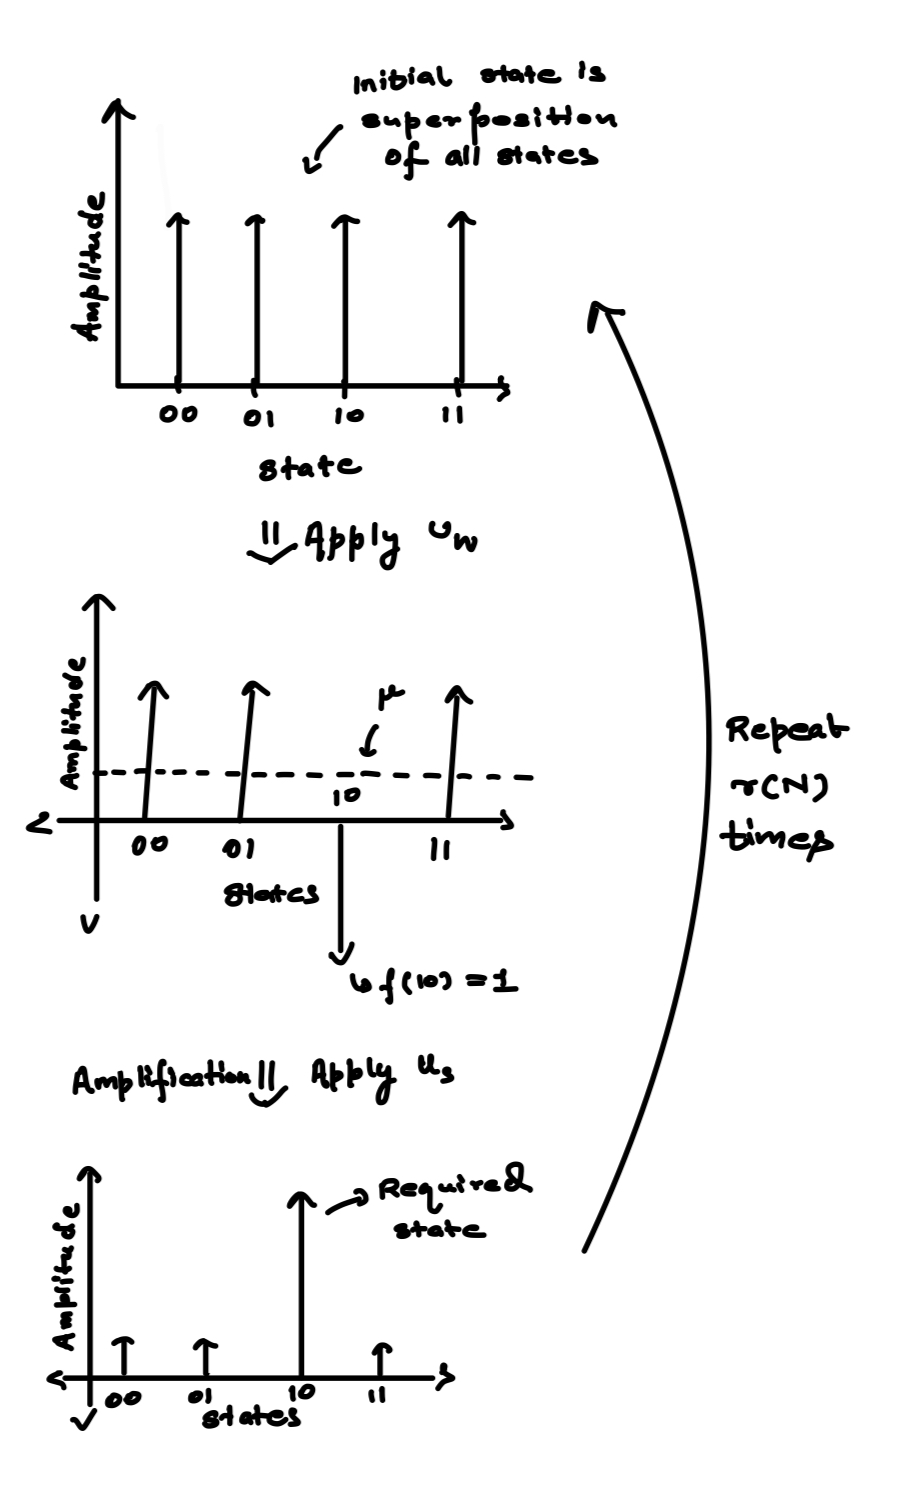
\includegraphics[width=0.9\textwidth]{pro.jpeg}
  \caption{Schematic of Grover's algorithm}
  \label{Schematic of Grover's algorithm}
\end{figure}

\subsection{Modification for many solutions:}

It is known that for oracles with at most one solution, the optimal number of iterations to apply is $\frac{\pi}{4}\sqrt{N}$, where N = $2^n$ is the size of the search space. However, it is also possible to handle oracles with multiple solutions. For
oracles with k solutions, the optimal number of iterations is instead $\frac{\pi}{4}\sqrt{\frac{N}{k}}$. To handle oracles with a possibly unknown number of solutions, the algorithm can be repeated using powers of two for k, which converges to an amortized complexity O($\sqrt{N}$).

Changing the number of iterations suffices to handle oracles with unknown numbers of solutions. Hence, in our
implementation, we restrict ourselves to the case of oracles with at most a single solution, since the circuit reduction
is independent of number of satisfying assignments in the Boolean formula. This modification allows us to find all possible solutions for the colouring.

\section{Coding in Qiskit:}

\subsection{The code:}

For the sake of simplicity and limited availability of hardward on actual quantum computer, I've considered 2-colouring of graphs, a.k.a. bipartite graphs.

Firstly, we import the required libraries of Qiskit, numpt and matplotlib:

\begin{lstlisting}[language=Python]
import numpy as np
from qiskit import QuantumCircuit, execute, transpile, Aer, IBMQ
from qiskit.visualization import *
import matplotlib.pyplot as plt
from qiskit.visualization import plot_histogram
from qiskit import QuantumRegister, ClassicalRegister, QuantumCircuit, IBMQ, execute
from qiskit import IBMQ, Aer, assemble, transpile
from qiskit.providers.ibmq import least_busy
from qiskit.visualization import plot_histogram


\end{lstlisting}

We then define a XOR gate function that takes a quantum circuit(qc), two inputs(a and b) and a output as arguments. Also, we define our graph in the edge-list format, where the pair [x, y] implies that there exists an edge between the vertices x and y. The variable num\_vertex denotes the total number of nodes in our graph.

\begin{lstlisting}[language=Python]
edge_list = [[0,1], [0,2], [1,3], [2,3]]    # This is the edge list
num_vertex = 4                              # This is the number of nodes

def XOR(qc, a, b, output):
# This function takes the quantum circuit 'qc' and make controlled-not gate with a and b as input
    qc.cx(a, output)
    qc.cx(b, output)
\end{lstlisting}

We define the variables for our circuit. Var\_qubits, edge\_qubits, output\_qubits, cbits and qc are the the qubits for the variable, edges, final output state, classical bit-length and the Quantum circuit, respectively.

\begin{lstlisting}[language=Python]
var_qubits = QuantumRegister(num_vertex, name='v')
edge_qubits = QuantumRegister(len(edge_list), name='c')
output_qubit = QuantumRegister(1, name='out')
cbits = ClassicalRegister(num_vertex, name='cbits')
qc = QuantumCircuit(var_qubits, edge_qubits, output_qubit, cbits)
\end{lstlisting}

We now define the edge colour oracle and apply the controlled-not gate between each ends of an edge using the XOR function defined above. We flip the output if all edges are satisfied which corresponds to the inversion in $U_\omega$ define about, i.e., $(-1)^{f(x)} \ket{x}$

\begin{lstlisting}[language=Python]
def edgeColor_oracle(qc, edge_list, edge_qubits):
    i = 0
    for edge in edge_list:
        XOR(qc, edge[0], edge[1], edge_qubits[i])
        i += 1
    # Flip 'output' bit if all edges are satisfied, mcx is the muli-control x operator
    qc.mcx(edge_qubits, output_qubit)
    # Reset the edges
    i = 0
    for edge in edge_list:
        XOR(qc, edge[0], edge[1], edge_qubits[i])
        i += 1

edgeColor_oracle(qc, edge_list, edge_qubits)
\end{lstlisting}

Now, we define the operation of the Grover's diffuser circuit, i.e. $U_s$ from above. We define the diffuser as a gate in revresible fashion. First apply the Hadamard gate on each qubit, which is followed by controlled-not operation on all the qubits. We then use the mcx gate similar to the one from oracle.

\begin{lstlisting}[language=Python]
def diffuser(nqubits):
    qc = QuantumCircuit(nqubits)
    # |s> -> |00..0>, prepare states
    for qubit in range(nqubits):
        qc.h(qubit)
    # Apply cnot |00..0> -> |11..1>
    for qubit in range(nqubits):
        qc.x(qubit)
    qc.h(nqubits-1)
    qc.mcx(list(range(nqubits-1)), nqubits-1)  # multi-controlled cnot
    qc.h(nqubits-1)
    # |11..1> -> |00..0>
    for qubit in range(nqubits):
        qc.x(qubit)
    # Go back to |00..0> -> |s>
    for qubit in range(nqubits):
        qc.h(qubit)
    # We create the greate U_s in this process
    U_s = qc.to_gate()
    U_s.name = "U$_s$"
    return U_s
\end{lstlisting}

Now, we finally prepare the qc output. Firstly, we initialise the output qubits. Then, we apply hadamard gate on var\_qubits to prepare the input state. Itrs represents the number of iterations for convergence to our solution. We then apply the oracle subroutine followed by the Grover's diffusion gate until our solution converges. Finally, we make the measurement and get our final result.

\begin{lstlisting}[language=Python]
# We first initialize the output as superposition of 0 states.
qc.initialize([1, -1]/np.sqrt(2), output_qubit)

# Initialize qubits in state |s>
qc.h(var_qubits)
qc.barrier()                    # For grouping the result

itrs = ((math.pi)*math.isqrt(num_vertex))/4 # Calculate the total number of iterations
itrs = int(math.ceil(itrs))                 # Take its int value

for itr in range(0, itrs):
    edgeColor_oracle(qc, edge_list, edge_qubits)
    qc.barrier() 
    # Apply our diffuser
    qc.append(diffuser(num_vertex), list(range(num_vertex)))

# Measure the variable qubits
qc.measure(var_qubits, cbits)

\end{lstlisting}

Finally, we process the result with the following code. 

\begin{lstlisting}[language=Python]
backend = Aer.get_backend('qasm_simulator') 
job = execute(qc, backend, shots = 1024) # Run qc circuit
result = job.result()    # Result object holds the final state
print(result)
counts = result.get_counts()  # Get the result in an array
plot_histogram(counts)        # Final plot of the result
\end{lstlisting}

Here, 1024 shots have been used for sampling, i.e. we use 1024 instances for sampling our final output.

In the above code, I used qasm\_simulator locally to run the simulation locally. You can get the 'API code' from your account and use the commented part from the code on my GitHub to run it on the actual IBM quantum computer. Since, sharing of API keys is not a safe practice, I've run the code on IBM's Manhattan quantum computer backend to get the results in the section 3.2.

\subsection{Results:}

The following results were obtained. The graphs have been visualized using [7].

1. Example of 2-colouring of graph with 4 nodes:

\begin{figure}[h]
  \centering
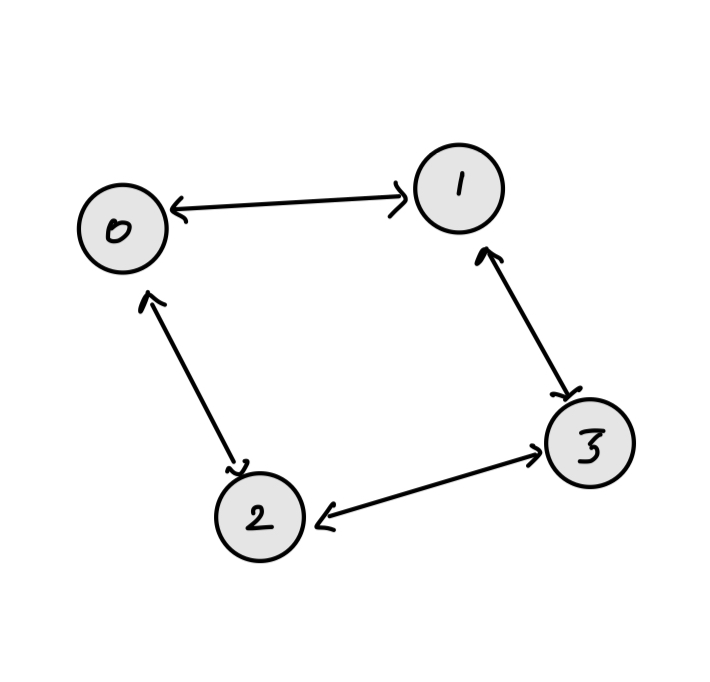
\includegraphics[width=0.4\textwidth]{Graph4.jpeg}
  \caption{Input graph with 4 nodes}
\end{figure}

\begin{figure}[h]
  \centering
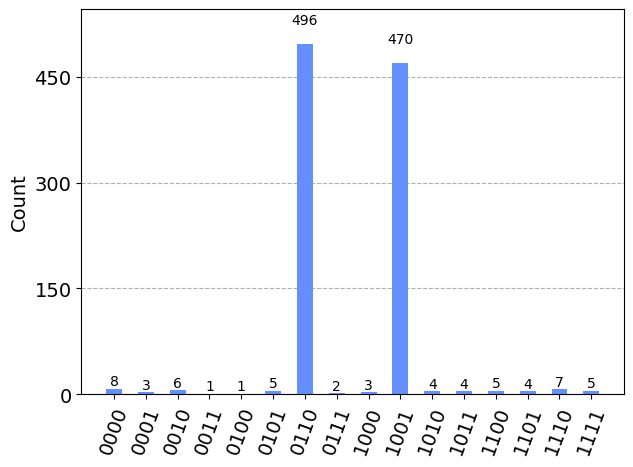
\includegraphics[width=0.4\textwidth]{output.png}
  \caption{Output after running Grover search}
\end{figure}

In the above output, 1 corresponds to one colour choice and 0 corresponds to another. Each bit is mapped to corresponding vertex number, respectively. Hence, the following two are the possibilities:

\begin{figure}[H]       
    \fbox{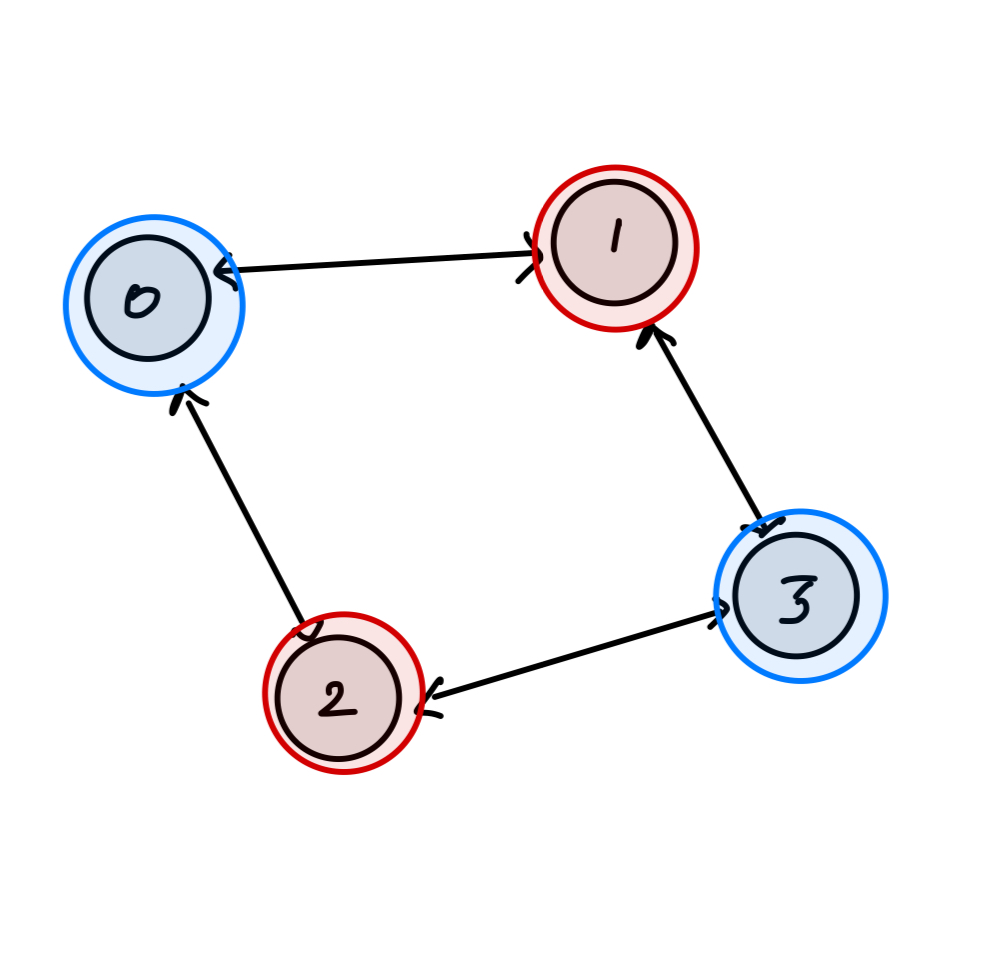
\includegraphics[width=0.4\textwidth]{Graph4-1.jpeg}}   
    \hspace{30px}
    \fbox{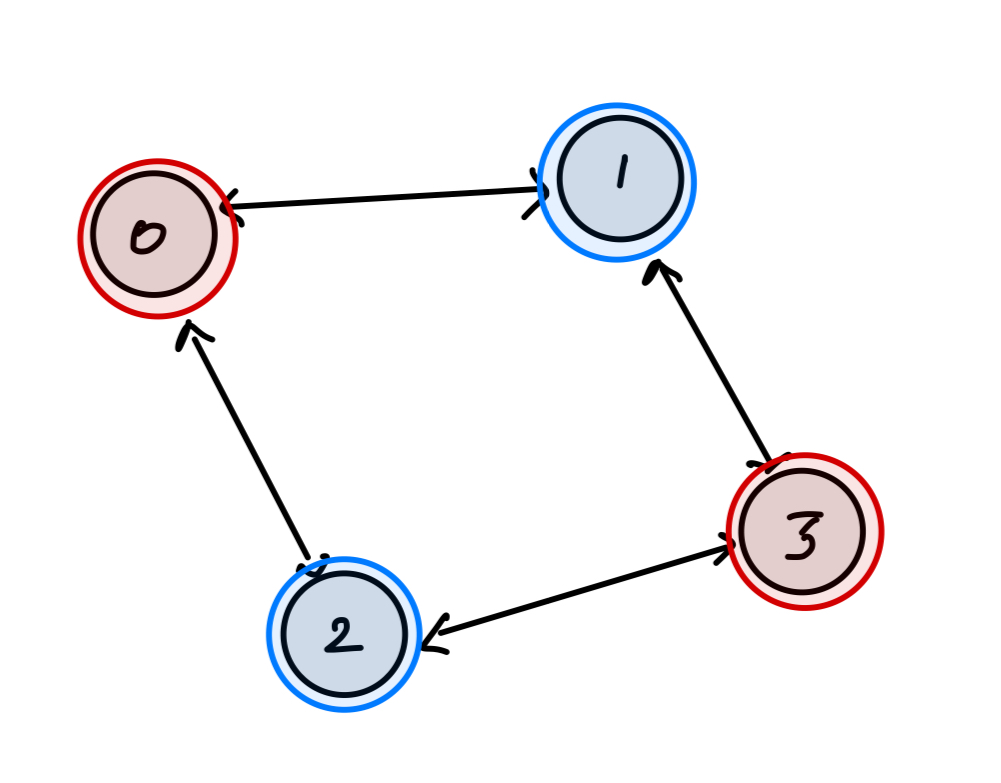
\includegraphics[width=0.4\textwidth]{Graph4-2.jpeg}}
    \hspace{30px}
    \caption{Possible 2-colourings of input graph}
\end{figure}

2. Example of 2-colouring of graph with 6 nodes:

\begin{figure}[h]
  \centering
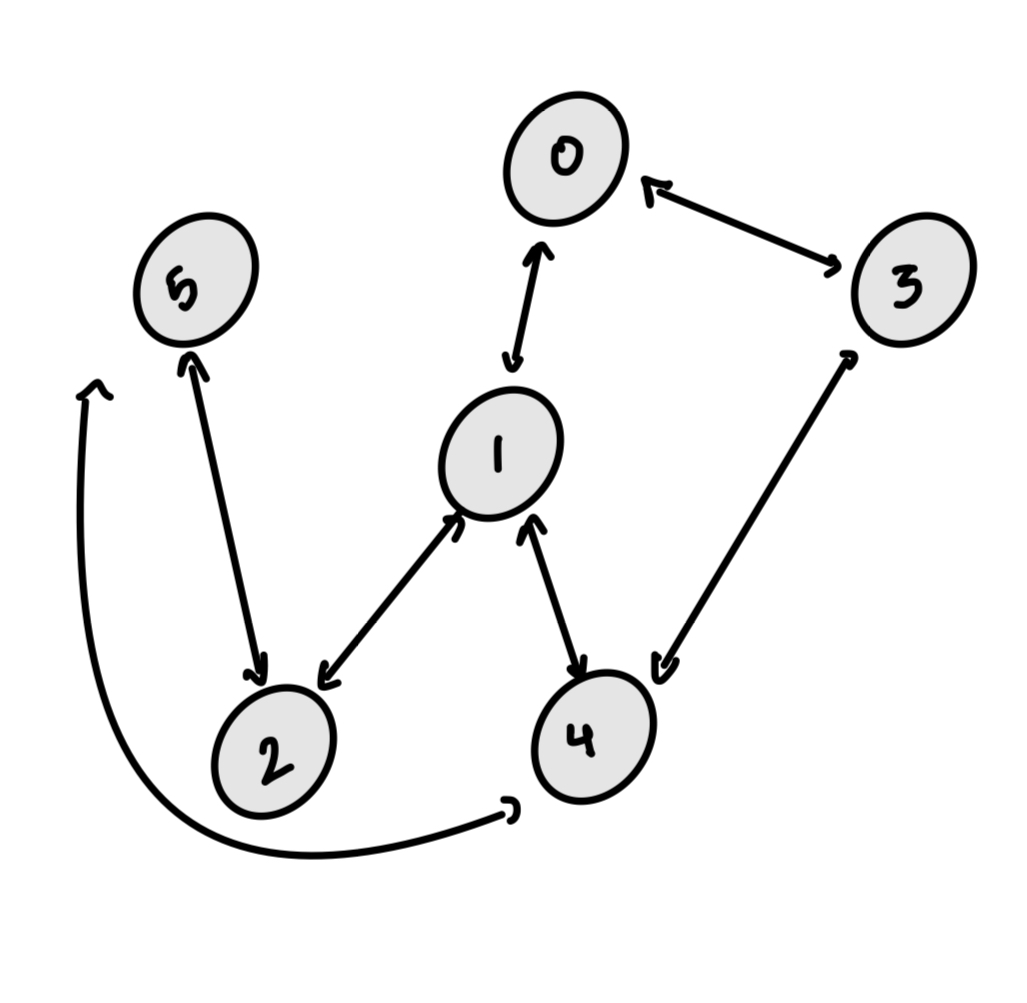
\includegraphics[width=0.4\textwidth]{graph6.jpeg}
  \caption{Input graph with 4 nodes}
\end{figure}

\begin{figure}[h]
  \centering
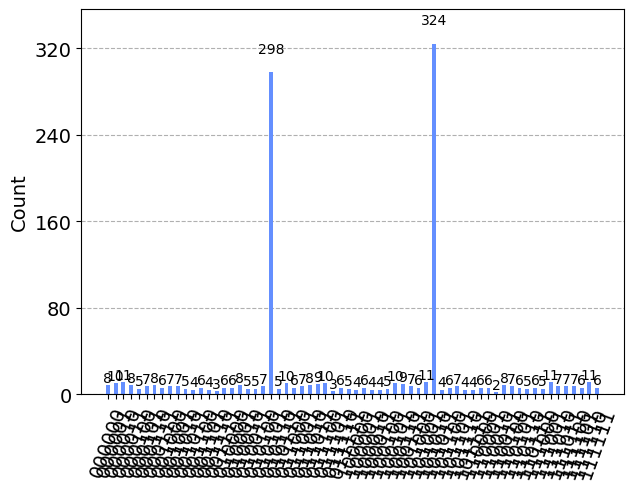
\includegraphics[width=0.4\textwidth]{output2.png}
  \caption{Output after running Grover search}
\end{figure}

In the above output, the peaks correspond to the bit-strings 101010 and 010101, respectively. The corresponding colourings are:

\begin{figure}[H]       
    \fbox{\includegraphics[width=0.4\textwidth]{Graph6-1.jpeg}}   
    \hspace{30px}
    \fbox{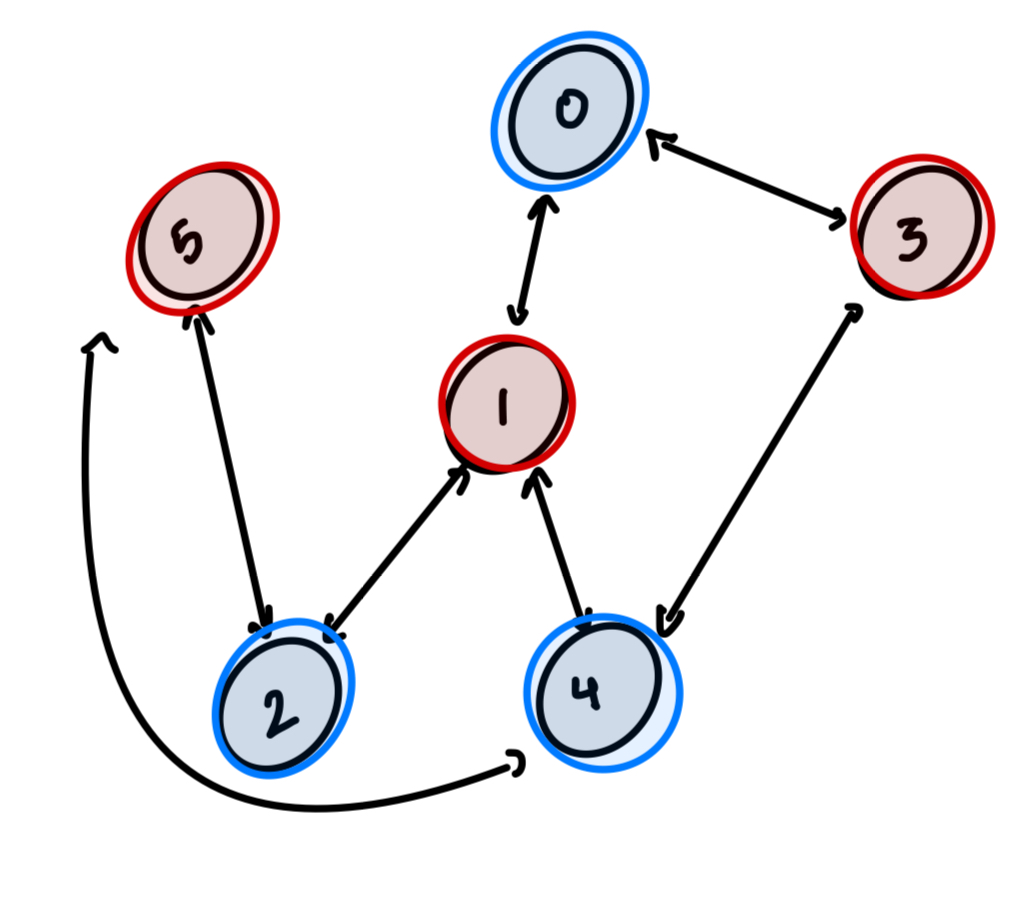
\includegraphics[width=0.4\textwidth]{Graph6-2.jpeg}}
    \hspace{30px}
    \caption{Possible 2-colourings of input graph}
\end{figure}

\section{Results, discussion and future improvements:}

It can be seen in the above examples, the quantum computer gives the correct bipartite coloring for the graph, the one where no two vertex connected by edges have the same colour! Hence, the Grover's algorithm was successful in finding the correct colouring of our graph in just O($N^{1/2}$) iterations, which is a massive speedup to classical methods of exhaustively searching through the solution space.

However, we encounter two major hurdle in current near-term quantum computers- the lack of quantum bits to support more complex cases, and large computational overhead. Hence, such computations as of now are not very helpful. Currently, I used n*k Qubits for the computations which grows very fast and it not practical. The future generation of fault-tolerant computers with better hardware might be able to speedup the process for practical instances of problems and veritication of solutions for NP-complete problems of practical interest.

\section{References and acknowledgements}

\begin{enumerate}
    \item \href{https://en.wikipedia.org/wiki/Graph_theory}{Wikipedia: Graph Theory}
    \item \href{https://en.wikipedia.org/wiki/Graph_coloring}{Wikipedia: Graph Colouring}
    \item \href{https://cse.iitkgp.ac.in/~palash/2018AlgoDesignAnalysis/SAT-3SAT.pdf }{K-SAT to 3-SAT}
    \item \href{https://en.wikipedia.org/wiki/Grover%27s_algorithm}{Wikipedia: Grover's algorithm}
    \item \href{https://research.ijcaonline.org/encc/number1/encc004.pdf}{K-colourability to 3-SAT}
    \item Descartes, Blanche, "A three colour problem", Eureka
    \item \href{https://csacademy.com/app/graph_editor/}{CSA's graph visualization tool}
\end{enumerate}

\section{Github link:}

The code can be found at \href{https://github.com/yashnator/Graph-colouring-with-Quantum-Computing}{This GitHub link}. You can uncomment the back-end part and add your API Key from IBM Qiskit's website to test the code on a Quantum computer.

\end{document}
